\chapter{Simmetrie}

Riprendiamo la discussione sulle simmetrie introdotta nella sezione \ref{sec: sim_intro}. 
Espandiamo il concetto di simmetria da un semplice cambio di visuale a vere e proprie trasformazioni di stati e osservabili, che mantengano sempre invariati i valori medi:
\[
    \Sigma\to \Sigma' \qquad \mathcal{A}\to \mathcal{A}' \qquad  \text{ t.c. } \expval{\mathcal{A}}_\Sigma  = \expval{\mathcal{A}'}_\Sigma
\]

Dal teorema di Wigner \ref{theo: Wigner} sappiamo che queste trasformazioni \(\tau\) sono indotte da operatori unitari o antiunitari \(U\), ma non garantisce l'unicità dell'operatore per simmetria.

\begin{theorem}
    Due operatori unitari o antiunitari \(U, \ U'\) inducono la stessa simmetria sse \(U ' = e^{i\theta}U\) .
\end{theorem}
\begin{proof}
    \((\impliedby) \) 
    \[
        \left[ \Psi \right]\to \left[ e^{i\theta}U \Psi\right]= \left[ \Psi \right] \quad A \to e^{i\theta}UAU^\dagger e ^{-i\theta}= UAU^\dagger
    \]
    \((\implies) \) supposto che \(\tau_U = \tau_{U'}: \ \ UAU^\dagger = U'AU'^\dagger\) abbiamo che:
    \[
       U^\dagger U A U^\dagger U'= U^\dagger U'A A'^\dagger U'  \implies AU^\dagger U'= U^\dagger U ' A
       \implies \left[ U^\dagger U', A \right]=0
    \] 
    Sfruttiamo il lemma: \(B\) t.c. \(\left[ B,A \right]= 0 , \ A \) a.a. \(\implies B = \lambda\mathbb{I}\).
    \[
        \implies U^\dagger U' = \lambda\mathbb{I} , \ \abs{\lambda} = 1 \implies U ' = e^{i\theta}U
    \]
\end{proof}
Perciò ogni trasformazione di simmetria \(\tau\) è indotta da un \textit{raggio operatore} (anti)unitario:
\[
    \left[ U_\tau \right]= \left\{ U \ \text{ (anti)unitario t.c. } U' = e^{i\theta}U , \ \theta \in \mathbb{R}\right\}
\]

\begin{remark}
    \(\mathbb{I}\) è simmetria, composizione di simmetrie \(\tau_1 \circ \tau_2\) è simmetria e \(\tau^{-1}\) è simmetria.
\end{remark}


\section{Gruppo di simmetria}
\begin{definition}
    Definiamo \textit{gruppo} \((G; \cdot )\) un insieme \(G\) dotato di un'operazione \(\cdot \) :
    \[
        \cdot : G \times G \to G \qquad (g,h)\to gh
    \]
    tale che:
    \begin{itemize}
        \item Associativa: \((gh)k= g(hk) \quad \forall\, g,h,k \in G\) .
        \item Esiste neutro: \(\exists 1 \in G :\ 1g = g1 = g \quad \forall \, g \in G\) .
        \item Esiste inverso: \(\forall \, g \in G , \ \exists\, g^{-1}\in G : \ gg^{-1}= 1 = g^{1}g\)
    \end{itemize}
\end{definition}
Se vale anche la proprietà commutativa \(gh = hg \ \forall\, g,h \in G\) allora il gruppo si dice \textit{abeliano}.
\begin{remark}
    Si dimostra che \(1\) e \(g^{-1}\) dato \(g\) sono unici.
\end{remark}

\begin{example}
    \((\mathbb{Z}; + ), \ (\mathbb{R}; +), (\mathbb{C}, +)\) sono gruppi abeliani. \\
    \((\mathbb{N}; +)\) non è un gruppo.
\end{example}
\begin{example}
    \(\left\{ \text{ matrici in } \mathbb{F} \text{ campo } n\times n \text{ invertibili } \right\}= GL(\mathbb{F}^n)\) , 
    \(V\) spazi vettoriali: \(GL(V)= \left\{ \text{ operatori lineari invertibili } A: V\to V\right\}\) sono gruppi con la composizione di matrici/funzioni.
\end{example}

Le simmetrie della fisica \(\tau\) sono un gruppo \(G\) rispetto all'operazione di composizione:
\[
    \tau \leftrightarrow \left[ U_\tau \right]; \quad id \leftrightarrow \left[ \mathbb{I} \right]  ;\quad \tau_1\circ \tau_2 \leftrightarrow \left[ U_{\tau_1} U_{\tau_2} \right]; \quad
    \tau^{-1}\leftrightarrow \left[ U^{-1}_\tau \right] = \left[ U^\dagger _\tau \right]
\]
Sto rappresentando il gruppo delle simmetrie della fisica attraverso gli operatori unitari.

\begin{definition}
    Dato un "gruppo astratto" \(G\) e uno spazio vettoriale \(V\) si dice \textit{rappresentazione} di \(G\) su \(V\) la mappa:
    \[
        \rho: G \to GL(V) \quad g \to \rho(g)
    \]
    tale che:
    \begin{itemize}
        \item \(\rho(1)= \mathbb{I}\)
        \item \(\rho(gh)= \rho(g)\rho(h)\)
        \item \(\rho(g^{-1}) = \rho(g)^{-1}\)
    \end{itemize}
    \((\rho, V)\) è detta \textit{rappresentazione lineare } di \(G\).
\end{definition}

\begin{example}
    \(G= \left\{ 1,i,,-1,-i \right\}\) è gruppo rispetto al prodotto. \(V \subseteq \mathbb{C}^2: \)
    \[
        \begin{pmatrix}
            1&0\\0&1
        \end{pmatrix} \quad
        \begin{pmatrix}
            0&-1\\1&0
        \end{pmatrix} \quad
        \begin{pmatrix}
            -1&0\\0&-1
        \end{pmatrix} \quad
        \begin{pmatrix}
            0&1\\-1&0
        \end{pmatrix} \quad
    \]
    è rappresentazione di \(G\) .
\end{example}

% 15 Lezione del 31/10/2025

Se \(V\) è spazio di Hilbert e \(\rho(g)\) è unitario \(\forall \, g \in G\), allora \(\rho\) è \textit{rappresentazione unitaria}.

Chiediamoci ora \(\rho: \tau\to \rho(\tau)= U_\tau\), dove scelgo \(U_\tau \) come rappresentante di \(\left[ U_\tau \right]\), è rappresentazione?\\
Possiamo sempre scegliere per \(\tau = id\) tra i \(\left[ \mathbb{I} \right] \) l'operatore \(\mathbb{I}\). Scelti \(U_{\tau_1}\) e \(U_{\tau_2}\),
si sceglie per \(\tau_3 =\tau_1 \circ \tau_2 \) il raggio operatore \(\left[ U_{\tau_3} \right]\) rappresentato da \(U_{\tau_3}= e^{i\theta_{12}}U_{\tau_1}U_{\tau_2}\)
non sempre esiste però \(U_{\tau_3}\) t.c. \(e^{i\theta_{12}}=1\) condizione necessaria per essere rappresentazione.

\begin{definition}
    Definiamo una \textit{rappresentazione proiettiva}, come una mappa \(\rho: G \to GL(V)\) tale che:
    \[
        \rho(1) = e^{i\alpha}\mathbb{I} \qquad \rho(gh)= e^{i\theta(g,h)} \rho(g)\rho(h)
    \]
\end{definition}

E allora posso fare scelte diverse: \( \rho : \tau \mapsto U'_\tau = e^{i\alpha(tau)}U_\tau\)
\[
    U'_{\tau_3} = e^{i\alpha_3} U_{\tau_3}= e^{i\alpha_3}e^{i\theta_{12}}U_{\tau_{1}}U_{\tau_2}= 
    e^{i\theta'_{12}}U'_{\tau_1}U'_{\tau_2}
\]
con \(\theta_{12}' = \theta_{12} + \alpha_{\tau_1} + \alpha_{\tau_2} - \alpha_{\tau_1\tau_2}\)
ma non si potrà sempre trovare una scelta con \(e^{i\theta(g,h)}=1 \ \forall\, g,h\) .

\begin{definition}
    \(\rho\) si dice genuinamente proiettiva se non esiste una ridefinizione che cancelli le fasi.
\end{definition}


\begin{example}
    \(\mathcal{H} = \mathbb{C}^2\)

    \[
        id = 
        \begin{pmatrix}
            1 & 0\\
            0 & 1
        \end{pmatrix}
        \qquad
        \tau_1 =
        \begin{pmatrix}
            0 & 1\\
            1 & 0
        \end{pmatrix}
        \qquad
        \tau_2 =
        \begin{pmatrix}
            0 & -i\\
            i & 0
        \end{pmatrix}
        \qquad
        \tau_3 =
        \begin{pmatrix}
            1 & 0\\
            0 & -1
        \end{pmatrix}
    \]

    \[
        \tau_1 \circ \tau_2 = \tau_2 \circ \tau_1 = \tau_3
        \qquad
        \tau_k \circ \tau_k = id
    \]

    \[
        U_1U_2 = iU_3, \qquad U_2U_1 = -iU_3, \qquad U_k^2 = \mathbb{I}
    \]

    Nessuna scelta di \(U_1, U_2, U_3\) soddisfa \(U_1U_2=U_3\) e \(U_k^2=\mathbb{I}\).
\end{example}

\begin{definition}
    Definiamo \textit{gruppo continuo ad un parametro}, gruppi che dipendono da un parametro come \(\left\{ \tau(s) \right\}_{s \in \mathbb{R}}\) tali che:
    \[
        \tau(0)= id\,;\qquad \tau(s)\circ \tau(s') = \tau(s+s')\,;\qquad\tau(s)^{-1} = \tau(-s )
    \]
\end{definition}

Gli \(U(s)\) che rappresetano \(\tau(s )\) sono sempre unitari: \(\forall \, s \in \mathbb{R}, \ U(s) = e^{i\theta}U(\frac{s}{2})U(\frac{s}{2})\).


\begin{theorem}
    Un gruppo a un parametro non ammette rappresentazione genuinamente proiettive.
\end{theorem}
E' sempre possibile, dunque, secgliere una rappresentazione tale che \(U(0)= \mathbb{I}, \  U(s)U(s')= U(s+s')\) .

Se considero \(s \) infinitesimo, posso sviluppare in Taylor:
\[
    U(s )\ket{\Psi}= U(0)\ket{\Psi}+ s \dv{U}{s} \eval_{s = 0} + \dots = \mathbb{I} - \frac{i}{\hbar}s Q    + \dots
\]
Dove è stato definito il \textit{generatore infinitesimo di trasformazioni} \(Q = i\hbar \dv{U}{s}\eval_{s =0}\).
\begin{remark}
    \(Q\) è hermitiano dato che deve valere \(U^\dagger(s)= U(-s)\).
\end{remark}


\begin{theorem}\label{theo: Stone}
    {\normalfont\textbf{di Stone}} Dato un gruppo a un parametro \(\left\{ U(s) \text{ unitari } , \ s \in \mathbb{R}\right\}\) tale che \(U(0)= \mathbb{I}\), \(U(s )U (s') = U(s+s')\) e sia continuo in \(s \), allora:
    \[
        Q\ket{\Psi} \equiv i\hbar \dv{s}U(s )\eval_{s=0}\ket{\Psi}    := i\hbar\lim_{s \to 0} \frac{U(s)\ket{\Psi}-\ket{\Psi}}{s}
    \]
    converge \(\forall\,\ket{\Psi}\in  D \subseteq \mathcal{H}, \ \overline{D}= \mathcal{H}\), \((Q,D)\) è a.a. e \(U(s )= e^{-\frac{i}{\hbar}sQ}\).\\
    Viceversa, dato un operatore a.a. \((Q, D)\) denso \(D \subseteq\mathcal{H}, \ \overline{D}= \mathcal{H}\) allora \(U(s)= e^{-\frac{i}{\hbar}sQ}\) è gruppo ad un parametro di oepratori unitari.
\end{theorem}

Consideriamo una simmetria a un parametro \(\tau(s ): A \to A(s )= U(s )A U(s )^\dagger \):
\[
    A(s) = 
    \left( \mathbb{I} - \frac{i}{\hbar}sQ + \dots \right)
    A
    \left( \mathbb{I} + \frac{i}{\hbar}sQ + \dots \right)
    = A - \frac{i}{\hbar}\left[ Q, A \right]s + \dots
\]

\[
   \implies  i\hbar \dv{}{s}\left( U(s)AU(s)^\dagger \right)\eval_{s=0} = \left[ Q, A \right]
\]
Se \(Q\) commuta con \(A\) allora \(A\) è invariante per la simmetria \(\tau(s )\).


\subsection{Traslazioni spaziali 1D}
Dall'omogeneità dello spazio, vogliamo studiare una simmetria \(\tau(a) \leftrightarrow \left[ U(a) \right]\rightsquigarrow U(a)\) che agisca nella seguente maniera:
\[
    U(a)\ket{\Psi}= \ket{\Psi'} \quad \Psi'(x)= \Psi(x-a) \quad X' = U(a)XU(a)^\dagger = X- a\mathbb{I} \quad U(a)P U(a)^\dagger = P
\]


\begin{figure}[h]
    \centering
    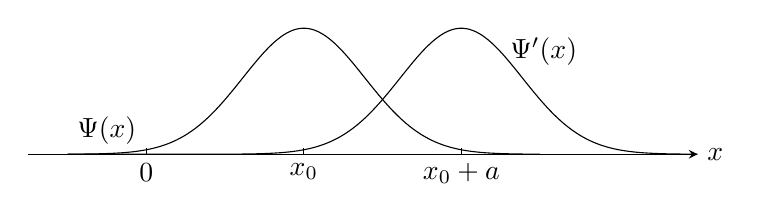
\begin{tikzpicture}[>=stealth]
        % assi
        \draw[->] (-0.5,0) -- (8,0) node[right] {$x$};
        % tacche e etichette
        \draw (1,0) -- (1,0.08) node[below,yshift=-2pt] {$0$};
        \draw (3,0) -- (3,0.08) node[below,yshift=-2pt] {$x_0$};
        \draw (5,0) -- (5,0.08) node[below,yshift=-2pt] {$x_0+a$};
        % profili d'onda (gaussiane stilizzate)
        \draw[smooth,domain=0:6,samples=200]
            plot(\x,{1.6*exp(-((\x-3)^2)/1.2)}) node[pos=0.28,above right] {$\Psi(x)$};
        \draw[smooth,domain=0:8,samples=200]
            plot(\x,{1.6*exp(-((\x-5)^2)/1.2)}) node[pos=0.78,above right , xshift = 5.5cm, yshift = 1cm] {$\Psi'(x)$};
    \end{tikzpicture}
    \caption{Traslazione di una funzione d'onda: $\Psi'(x)=\Psi(x-a)$.}
    \label{fig:traslazione-1d}
\end{figure}

L'operatore \(U(a)\) trasla la funzione d'onda, mentre l'operatore \(X'\) trasla il sistema di riferimento,
quindi i valori medi misurati sono gli stessi. 
Mentre l'operatore momento rimane invariato come ci si aspetta da una traslazione spaziale.

Per il teorema di Stone \ref{theo: Stone} deve esistere un generatore infinitesimo della trasformazione:
\[
    \bra{x} i\hbar\dv{a}U(a)\eval_{0}\ket{\Psi}= i\hbar \lim_{a\to 0 }   \frac{\bra{x}U(a)\ket{\Psi}-\braket{x}{\Psi}}{a}= i\hbar\lim_{a\to0 }\frac{\Psi(x-a)-\Psi(x)}{a} = -i\hbar \dv{x}\Psi(x)
\]
Che, in rappresentazione \(x\), corrisponde all'operatore momento \(P\) che dunque è il generatore infinitesimo di traslazioni:
\begin{equation}
    U(a) = e^{-\frac{i}{\hbar}aP}
\end{equation}


% Commutatore canonico e traslazioni generate da P
Supponiamo di partire da un sistema quantistico con
\[
    [Q,P]= i\hbar , \qquad Q,P \text{ a.a.}
\]
(coerente con la quantizzazione del corrispondente sistema classico).
Dato che \(P\) è a.a., l’operatore
\[
    U(a)\equiv e^{-\frac{i}{\hbar}aP}, \qquad a\in\mathbb{R},
\]
è un gruppo uniparametrico di operatori unitari.

\begin{equation}
    [Q,U(a)] =\left[ Q, e^{-\frac{i}{\hbar}aP} \right]     = aU(a).
\end{equation}


Sia \(\ket{q}\) un autovettore (generalizzato) di \(Q\): \(Q\ket{q}=q\ket{q}\): 
\[
    Q\,U(a)\ket{q}= \bigl(U(a)Q + aU(a)\bigr)\ket{q}
                 = (q+a)\,U(a)\ket{q}.
\]
Dunque \(U(a)\ket{q}\) è ancora autovettore di \(Q\) con autovalore \(q+a\).
Poiché \(a\in\mathbb{R}\) è arbitrario, segue che lo spettro di \(Q\) è traslato di qualsiasi quantità reale:
\[
    q\in\sigma(Q)\ \Longrightarrow\ q+a\in\sigma(Q)\ \ \forall\,a\in\mathbb{R}
    \quad\Longrightarrow\quad \sigma(Q)=\mathbb{R}.
\]


Gli operatori \(U(a)=e^{-\frac{i}{\hbar}aP}\) realizzano le traslazioni di \(Q\);
equivalentemente, \(P\) è il generatore infinitesimo delle traslazioni della variabile coniugata a \(Q\).


\subsection{Traslazioni spaziali in 3D}

Sia \(\vec a=(a_x,a_y,a_z)\). Le traslazioni formano un gruppo abeliano a tre parametri:
\[
\tau(\vec a)\circ\tau(\vec b)=\tau(\vec a+\vec b)=\tau(\vec b)\circ \tau(\vec a)\,.
\]
La rappresentazione unitaria \(U(\vec a)\) agisce su stati e osservabili come
\[
\ket{\Psi'}=U(\vec a)\ket{\Psi}, 
\qquad \Psi'(\vec x)=\Psi(\vec x-\vec a), 
\qquad U(\vec a)\,\vec X\,U(\vec a)^\dagger=\vec X-\vec a, 
\qquad U(\vec a)\,\vec P\,U(\vec a)^\dagger=\vec P .
\]

I generatori infinitesimi lungo gli assi sono \(P_x,P_y,P_z\) e, in generale,
\[
P_i \;=\; i\hbar\,\pdv{U(\vec a)}{a_i}\bigg|_{\vec a=0},\qquad i=x,y,z.
\]
Per una traslazione nella direzione unitaria \(\hat n\):
\[
i\hbar\,\dv{s}U(s\hat n)\bigg|_{s=0}= \vec P\!\cdot\!\hat n,
\]
e, dato un vettore arbitrario \(\vec a\),
\[
i\hbar\,\dv{s}U(s\vec a)\bigg|_{s=0}= \vec P\!\cdot\!\vec a.
\]

Dal teorema di Stone segue dunque
\[
U(\vec a)=\exp\!\left(-\frac{i}{\hbar}\,\vec P\!\cdot\!\vec a\right).
\]
Poiché \([P_i,P_j]=0\) si può fattorizzare (l’ordine è irrilevante):
\[
U(\vec a)=e^{-\frac{i}{\hbar}P_x a_x}\,e^{-\frac{i}{\hbar}P_y a_y}\,e^{-\frac{i}{\hbar}P_z a_z}.
\]












\section{Si vedrà}
% Da fare Lezione del 04/10/0225

\subsubsection{Rototraslazioni}

\(g = (R, \vec{a})= (\mathbb{I}, \vec{a})(R,0)\)\\
\(\vec{x}'= (R, \vec{a})\vec{x}= R\vec{x}+ \vec{a}\)
\((R_1,\vec{a_1})(R_2, \vec{a_2})\vec{x}= (R _1, \vec{a})(R_2\vec{x}+\vec{a_2})= R_1R_2\vec{x}+ R_1\vec{a}+ \vec{a_1}= (R_1R_2, R_1\vec{a_2}+\vec{a_1})\)
\(1d = (\mathbb{I},0)\)
l'inversa è \((R,\vec{a})^{-1}= (R^{-1}, -R^{-1}\vec{a})\):
\[
    (R, \vec{a})(R^{-1}, R^{-1}\vec{a}) = (\mathbb{I}, - RR^{-1}\vec{a}+\vec{a})= (\mathbb{I},0)
\]

\(U_{(R, \vec{a})}= U_{\vec{a}}U_{R(\vec{\omega})}= e^{-\frac{i}{\hbar}\vec{P}\cdot\vec{a}}e^{-\frac{i}{\hbar}\vec{\omega}\cdot\vec{j}}\)

\(\left[ J_i, J_j  \right]= i\hbar \sum_k\epsilon_{ijk}J_k\)
\[
    \left[ P_i, P_j \right] =0 \qquad \left[ J_i, P_j\right] = i\hbar \sum_k    \epsilon_{ijk}P_k
\]




\subsubsection{Traslazioni temporali}
Consideriamo \(\ket{\Psi(t)}\) soluzione equazione di Schrödinger.
\(\forall t.  \quad \ket{\Psi'(t)}= W\ket{\Psi(t)}\)
E' ancora soluzione dell'eq di Schödinger?
\[
    i\hbar\dv{t}W\ket{\Psi(t)} =   W i\hbar \dv{t}\ket{\Psi(t)} = W H(t)\ket{\Psi(t)}
\]
Questo è uguale a \(H(t)W\ket{\Psi(t)}\) sse \(\left[ W, H(t) \right]=0\)

Definiamo il \textit{gruppo di simmetrie della dinamica} come:
\[
    G_d = \left\{ W \text{ unitari }  : \left[ W, H \right]=0 \right\}
\]
Questo è equivalente a \(WHW^\dagger= H\) e se \(W\) è unitario allora \(\left[ W, U(t,t_0) \right]=0\)

Nella visuale di Heisenberg, con \(A_h(t)= U(t-t_0)^\dagger A_s U(t-t_0)\)
se \(W \in G_d\) vale:
\[
    WA_h(t)W^\dagger = U(t-t_0)^\dagger W A_s W^\dagger U(t-t_0)
\]

\(W(s)= e^{-\frac{i}{\hbar}sQ}\) vale:
\[
    \left[ W(s), H \right]= 0 \ \forall\, s \iff \left[ Q, H \right]    =0
\]

\begin{theorem}
    di Noether in MQ\\
    \(H\) invariante per simmetria generata da \(Q\) a.a. sse \(Q\) è quantità conservata 
\end{theorem}

